\documentclass[titlepage]{article}
\usepackage{graphicx}
\usepackage{amsmath}

% 设置A4纸
\usepackage[a4paper]{geometry}  

% 文档信息
\title{\textbf{Advanced Control for Robotics: Homework \#1}}
\author{Shang Yangxing}
\date{\today}

\begin{document}

\maketitle

\section{ODE and Its Simulation}

\subsection{Equation of Pendulum Motion}

\begin{figure}[htbp]
    \centering
    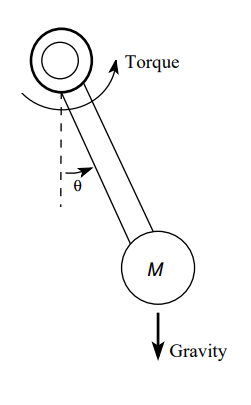
\includegraphics[width=.3\textwidth]{img/pendulum.png}
    \caption{pendulum model}
    \label{fig:pendulum}
\end{figure}

By applying the Newton's law of dynamics, a pendulum with no external force can be formulated as:

\begin{equation}
    ml^2 \ddot{\theta} + mgl \sin{\theta} - T = 0
\end{equation}

in which:

\quad $m$ is mass of the ball

\quad $l$ is length of the rod

\quad $g$ is the gravitational constant

\quad $\theta$ is angle between the rod and the vertical axis, which is also the system output $y$

\quad $T$ is torque of the joint, which is also the control input $u$



\section{Matrix calculus}
\section{Inner product}
\section{Some linear algebra}
\section{Gradient Flow}

\end{document}